\section{Task 3: Domain Generalization}

\subsection{Experimental Setup}
% Brief 2-3 sentence overview: same PACS protocol as Task 2 (Photo / Art Painting / Cartoon
% labelled sources), but Sketch is never loaded until the final evaluation script. ERM is
% the unchanged Task 2 Source-only checkpoint. DAN-DG adds the average pairwise MMD^2 over
% the three source pairs on the 512-d pre-head feature (same three RBF kernels as Task 2,
% lambda_DG = 1); SAM uses non-adaptive SAM with rho = 0.05 on AdamW. Same splits, optimiser,
% epoch budget, patience, 8 images per source domain per batch, and seed 6304; every
% checkpoint selected on mean source-validation macro-F1. Controlled study: lambda_DG in
% {0.1, 1, 10}.

\begin{table}[h]
  \caption{Source validation accuracy / macro-F1 (\%) per domain, with mean and worst, for ERM, DAN-DG and SAM, and the $\lambda_{\mathrm{DG}}$ study below the rule. Checkpoints were selected on mean macro-F1.}
  \label{tab:task3_source}
  \centering
  \small
  \setlength{\tabcolsep}{3pt}
  \begin{tabular}{lccccc}
    \toprule
    \textbf{Method} & Photo & Art & Cartoon & Mean & Worst \\
    \midrule
    ERM                                & 96.11 / 95.53 & 92.68 / 92.64 & 94.67 / 95.37 & 94.49 / 94.51 & 92.68 / 92.64 \\
    DAN-DG ($\lambda_{\mathrm{DG}}=1$) & 94.31 / 93.24 & 89.02 / 89.35 & 92.11 / 92.09 & 91.82 / 91.56 & 89.02 / 89.35 \\
    SAM ($\rho=0.05$)                  & 97.31 / 96.77 & 92.44 / 92.34 & 95.74 / 96.23 & 95.16 / 95.12 & 92.44 / 92.34 \\
    \midrule
    \multicolumn{6}{l}{\textit{Controlled study: alignment strength $\lambda_{\mathrm{DG}}$ in DAN-DG}} \\
    DAN-DG ($\lambda_{\mathrm{DG}}=0.1$) & 95.51 / 94.67 & 91.46 / 91.24 & 91.68 / 92.17 & 92.89 / 92.69 & 91.46 / 91.24 \\
    DAN-DG ($\lambda_{\mathrm{DG}}=10$)  & 41.32 / 21.54 & 25.12 / 15.39 & 18.12 / 11.24 & 28.19 / 16.06 & 18.12 / 11.24 \\
    \bottomrule
  \end{tabular}
\end{table}

\begin{table}[h]
  \caption{Sketch accuracy and macro-F1, change against ERM (pp), source-domain separability (3-way probe, chance 33.3\%) and the sharpness proxy: validation loss $\mathcal L$, loss after a radius-0.05 ascent step $\mathcal L_{+\epsilon}$, and their difference $\Delta_{\mathrm{sharp}}$ (96 images). Plots: Appendix Figs.~\ref{fig:task3_alignment} and \ref{fig:task3_diagnostics}.}
  \label{tab:task3_target}
  \centering
  \small
  \setlength{\tabcolsep}{4pt}
  \begin{tabular}{lcccccccc}
    \toprule
    & \multicolumn{4}{c}{\textbf{Sketch}} & & \multicolumn{3}{c}{\textbf{Sharpness proxy}} \\
    \cmidrule(lr){2-5} \cmidrule(lr){7-9}
    \textbf{Method} & Acc & Macro-F1 & $\Delta$Acc & $\Delta$F1 & \textbf{Sep.} & $\mathcal L$ & $\mathcal L_{+\epsilon}$ & $\Delta_{\mathrm{sharp}}$ \\
    \midrule
    ERM                                & 55.71 & 55.90 & ---       & ---       & 86.38 & 0.192 & 0.792 & 0.600 \\
    DAN-DG ($\lambda_{\mathrm{DG}}=1$) & 68.44 & 72.37 & $+12.73$  & $+16.46$  & 80.07 & 0.217 & 0.849 & 0.631 \\
    SAM ($\rho=0.05$)                  & 64.55 & 67.64 & $+8.83$   & $+11.74$  & 86.38 & 0.073 & 0.214 & 0.141 \\
    \midrule
    \multicolumn{9}{l}{\textit{Controlled study: alignment strength $\lambda_{\mathrm{DG}}$ in DAN-DG}} \\
    DAN-DG ($\lambda_{\mathrm{DG}}=0.1$) & 71.70 & 72.63 & $+15.98$ & $+16.73$ & 81.40 & 0.150 & 0.887 & 0.737 \\
    DAN-DG ($\lambda_{\mathrm{DG}}=10$)  & 10.56 & 7.84  & $-45.15$ & $-48.06$ & 48.84 & 1.855 & 4.103 & 2.248 \\
    \bottomrule
  \end{tabular}
\end{table}

\subsection{Source Validation as a Predictor of Sketch Performance}



\begin{table}[t]
  \caption{Per-class Sketch accuracy (\%) with the change against ERM (pp) in brackets, including target-aware DAN from Task 2. Plots: Appendix Figs.~\ref{fig:task3_alignment} and \ref{fig:task3_vs_task2}.}
  \label{tab:task3_per_class}
  \centering
  \small
  \setlength{\tabcolsep}{2.5pt}
  \begin{tabular}{lcccccc}
    \toprule
    & & & \multicolumn{3}{c}{\textbf{Task 3}} & \textbf{Task 2} \\
    \cmidrule(lr){4-6} \cmidrule(lr){7-7}
    \textbf{Class} & Support & ERM & DAN-DG ($\lambda{=}1$) & SAM & DAN-DG ($\lambda{=}10$) & DAN \\
    \midrule
    \texttt{dog} & 772 & 36.79 & 36.66 ($-0.13$) & 30.18 ($-6.61$) & 11.79 ($-25.00$) & 63.60 ($+26.81$) \\
    \texttt{elephant} & 740 & 88.78 & 96.22 ($+7.43$) & 98.51 ($+9.73$) & 30.41 ($-58.38$) & 87.16 ($-1.62$) \\
    \texttt{giraffe} & 753 & 23.51 & 44.89 ($+21.38$) & 56.31 ($+32.80$) & 0.00 ($-23.51$) & 51.39 ($+27.89$) \\
    \texttt{guitar} & 608 & 83.06 & 95.56 ($+12.50$) & 85.36 ($+2.30$) & 0.66 ($-82.40$) & 84.87 ($+1.81$) \\
    \texttt{horse} & 816 & 45.59 & 73.04 ($+27.45$) & 55.64 ($+10.05$) & 0.00 ($-45.59$) & 47.67 ($+2.08$) \\
    \texttt{house} & 80 & 45.00 & 93.75 ($+48.75$) & 81.25 ($+36.25$) & 63.75 ($+18.75$) & 100.00 ($+55.00$) \\
    \texttt{person} & 160 & 98.75 & 65.00 ($-33.75$) & 70.00 ($-28.75$) & 27.50 ($-71.25$) & 97.50 ($-1.25$) \\
    \bottomrule
  \end{tabular}
\end{table}

Good performance on the source domain does not guarantee good performance on the target domain, and this is visible via the results (Tables~\ref{tab:task3_source} and~\ref{tab:task3_target}). Their worst-performing source macro-F1 is 89.35 and 92.34, respectively. While establishing a possible link between the validation numbers of source domains and the test numbers of the target domains, ERM, as anticipated, performed worst in the target domain, whereas DAN-DG has the lowest mean source accuracy of 91.82 and best target accuracy/macro-F1 of 68.44/72.37. SAM has performed the highest mean source accuracy of 95.16, but still its target accuracy is 3.89 points lower than DAN-DG. Therefore, it is difficult to establish that source validation performance reliably predicts performance on Sketch.

ERM performs very poorly on Sketch for giraffe, dog, horse, and house, with accuracies of 23.51\%, 36.79\%, 45.59\%, and 45.00\%, whereas in the case of DAN-DG, 5 out of 7 classes gained points (house by 48.75 points, horse by 27.45, giraffe by 21.38, and guitar by 12.50). However, for the person, the performance declined by 33.75 points. Therefore, high aggregate source performance hides substantial target-specific class failures, particularly the degradation of person and the continued difficulty of dog recognition.

The art domain is recorded as the worst across all three methods.

\FloatBarrier
\subsection{Source-Domain Invariance and Class-Discriminative Information}

\begin{figure}[t]
  \centering
  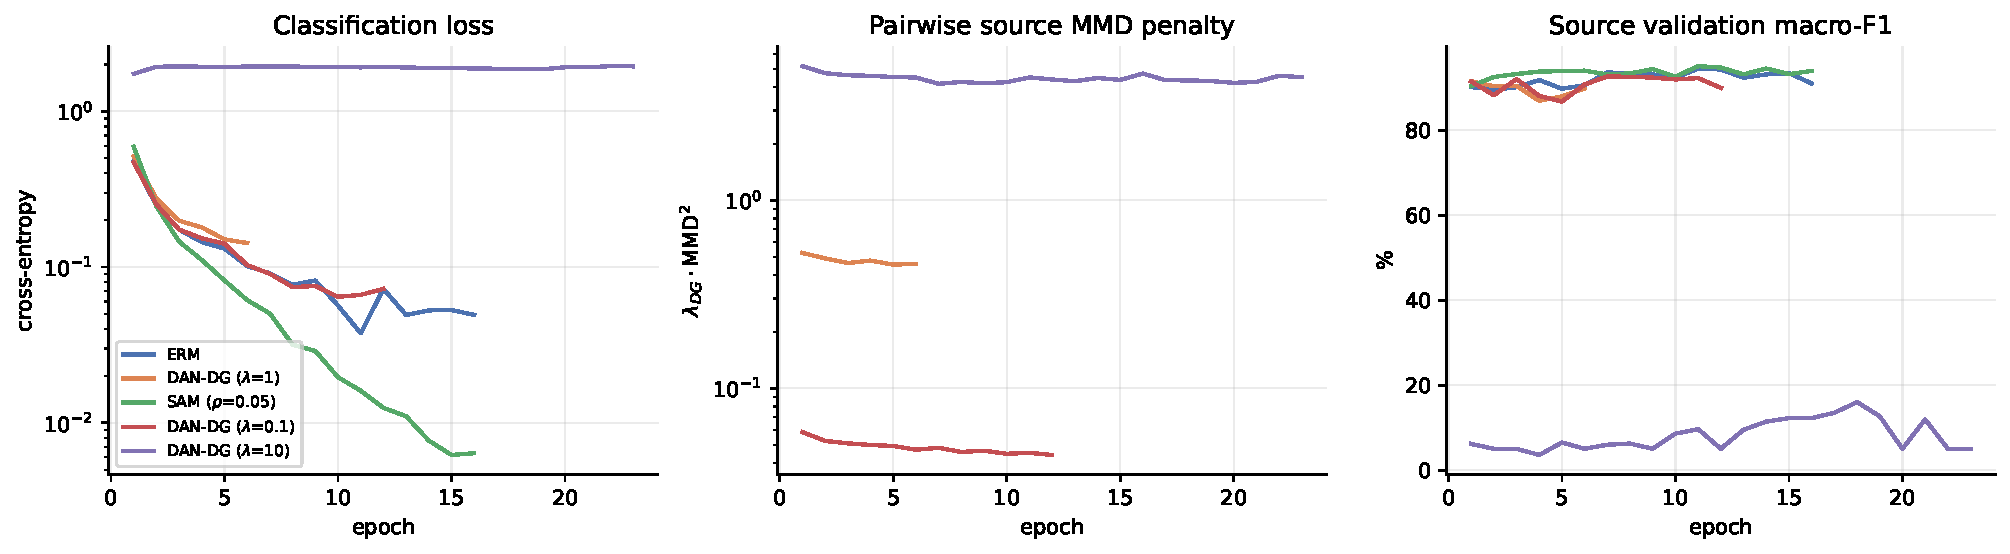
\includegraphics[width=\textwidth]{figures/task3/fig1_training_curves.pdf}
  \caption{(a) Classification loss, (b) weighted pairwise source MMD penalty for DAN-DG, (c) mean source-validation macro-F1. ERM is the reused Task 2 run; curves end at early stopping.}
  \label{fig:task3_training}
\end{figure}



DAN-DG made the observed source domains slightly less distinguishable, as shown by the source-domain separability score, which decreases to 80.07\% compared with 86.38\% under ERM. Its performance on Sketch also got better, and it reported an increase in macro-F1 from 55.90 to 72.37. These numbers appear to support the claim; however, the results change drastically when $\lambda_{\mathrm{DG}}$ is increased to 10. The separability score fell to 48.84\%, but the macro-F1 on both the Sketch and the source just collapsed to 7.84\% and 16.06\%, respectively. Class-wise, 6 out of 7 classes lost substantial points: guitar fell by 82.40 points, person by 71.25, elephant by 58.38, and both giraffe and horse reached 0\% accuracy. Moreover, in the case of SAM and ERM, the separability is identical at 86.38\%, yet SAM's Sketch macro-F1 is 67.64 against ERM's 55.90. This suggests that excessive source alignment does remove domain-discriminative features, making domains more difficult to distinguish; however, at the same time, it destroys the core semantic structure required for classification. Therefore, moderate invariance among the domains partially improves Sketch recognition, while a stronger push results in loss of critical class-discriminative information, resulting in poor performance on the target domain.

\FloatBarrier
\subsection{Local Stability and Sketch Performance}



A lower common sharpness proxy under given perturbation partially supports the claim about local stability, but it does not establish that the overall loss surface is flatter and will generalize better on any domain shifts. With SAM perturbation the loss increased by just 0.141, as compared to ERM and DAN-DG, which reported a change of 0.600 and 0.631, respectively. Therefore, the local stability ranking is
\[ \text{SAM} < \text{ERM} < \text{DAN-DG}. \]
However, it does not establish that the local stability ranking enables better performance on the target domain, because on the target domain the performance of each model is
\[ \text{DAN-DG} > \text{SAM} > \text{ERM}. \]
DAN-DG reported the highest sensitivity to a minor perturbation; however, its Sketch macro-F1 is the highest (72.37\%), whereas SAM is much flatter as per the proxy ranking, but it reaches 67.64\%. Nevertheless, SAM does improve over ERM by 8.83 accuracy points and 11.74 macro-F1 points, suggesting that local parameter stability may contribute to some extent to better generalization, but it is difficult to confirm that in every setting SAM will result in better performance on target domains.

\FloatBarrier
\subsection{Target-Aware DAN versus Target-Free DAN-DG}

Both methods improve substantially over the shared ERM baseline (Table~\ref{tab:task3_target_access})

\begin{table}[h]
  \caption{Target-aware DAN (Task 2) and target-free DAN-DG (Task 3) against the shared ERM checkpoint.}
  \label{tab:task3_target_access}
  \centering
  \small
  \begin{tabular}{llcc}
    \toprule
    \textbf{Method} & \textbf{Training alignment} & \textbf{Sketch accuracy} & \textbf{Sketch F1} \\
    \midrule
    ERM           & None                            & 55.71\% & 55.90\% \\
    Task 2 DAN    & Source versus unlabeled Sketch  & 67.80\% & 66.84\% \\
    Task 3 DAN-DG & Pairwise observed sources only  & 68.44\% & 72.37\% \\
    \bottomrule
  \end{tabular}
\end{table}

DAN used unlabeled Sketch data to align the source features and improved over ERM by 12.09 accuracy points and 10.93 macro-F1 points. DAN-DG, which never had access to the target data (sketches) during training, improved by 12.73 accuracy points and 16.46 macro-F1 points. DAN-DG exceeds target-aware DAN by 0.64 accuracy points and 5.53 macro-F1 points.

This suggests that access to unlabeled Sketch data did not provide a substantial empirical advantage. Instead, it highlights that DAN-DG was able to learn the cross-domain invariances, which resulted in source-target alignment. However, this does not establish that unlabeled Sketch data has no value, and several limitations prevent this from being a complete causal attribution.



The whole experiment is limited to a single seed, 6304, a different seed might have produced different results.

DAN and DAN-DG work on different distributions; the DAN objective aligns source and target domain features given by  \(\mathcal L_{\mathrm{align}}^{\mathrm{DAN}} = \operatorname{MMD}^2 \left( F(X_P\cup X_A\cup X_C), F(X_S) \right).\) whereas DAN-DG tries to learn invariances among the source domains:
\[ \mathcal L_{\mathrm{align}}^{\mathrm{DAN-DG}} = \frac{ \operatorname{MMD}^2(P,A) + \operatorname{MMD}^2(P,C) + \operatorname{MMD}^2(A,C) }{3}. \]
In DAN, the pooled comparison between the source and target can hide the differences between the individual source domains; however, the pairwise terms in DAN-DG ensure that these differences are accounted for.
